\section{Introduction}

This report shows the analysis we made over the shopping sessions registered by a supermarket; the goal is to understand the customers' behavior and to define different customer profiles.

\textbf{Don't know if we want to keep this introduction}
\pagebreak

\section{Data Understanding}

The dataset contains informations about the purchases of each customer of the supermarket. The dataset contains \textbf{471910} rows, each of one divided into \textbf{8} columns; each entry represents the purchase of a product by a customer, and it comprehends also informations about the date of the transaction, the price of the product and the quantity purchased.\\
A key information we extracted from the dataset, based on the products descriptions and the frequency of purchases per customer, is that the supermarket in question is not a food store, but instead a grocery store, that sells in particular fast-moving consumer goods.

\subsection{Data Semantics}

In this section, we describe the semantic of each attribute, providing also some statistics about them.

\textbf{BasketID} \\
A code that identifies a shopping session for a customer. It remains the same for all the rows that indicate different products inside a single session.\\
We have \textbf{22190} distinct Basket IDs.\\
We define \emph{good} \textbf{BasketID} as a six digit code, instead a \emph{bad} \textbf{BasketID} is composed by a character, \emph{C} or \emph{A}, followed by a six digit code.

\textbf{BasketDate}\\
The date and time of a transaction. Basket Dates that correspond to the same Basket ID have the same value.\\
The dates range from 2010 to 2011, while the times range from 6 to 21.

\textbf{Sale}\\
A numeric attribute that indicates the price of a product.
Since there is no currency associated with the sale price, we assume that it is always the same.

\textbf{CustomerID}\\
A code that identifies a customer. It is a five-digit code.\\
We have \textbf{4372} unique customer IDs, with some \emph{NULL} values.

\textbf{CustomerCountry}\\
A categorical attribute that indicates the country of origin of each customer.\\
We have \textbf{37} different countries.

\textbf{ProdID}\\
A code that identifies a product.\\
It most cases, it is a five-digit string; sometimes, it has a letter at the end, while other times it is a string of characters.\\
We have \textbf{3953} distinct Product IDs.
We define \emph{good} \textbf{ProdID} as a five digit code, possibly followed by a variable number of characters; everything else, which are strings followed by some numbers, is labelled as a \emph{bad} \textbf{ProdID}.

\textbf{ProdDescr}\\  
A string with a description of a product.\\
We have \textbf{4097} unique Product Descriptions, with some \emph{NULL} values.

\textbf{Qta}\\
A numeric attribute that represents the purchased quantity for each product.

\subsection{Assessing Data Quality}
Now, we describe a deeper analysis to assess the quality of data.\\
First, we checked for duplicate rows, and we found a total of \textbf{5232} duplicate records. Since each row represents a single purchase from a customer in a specific date, we have considered these duplicates as errors, and so we decided to drop them. After this correction, we have a dataset consisting of \textbf{466678} records.

Then, we focused on the missing values; in the dataset, we have only two columns with some \emph{NULL} values; in particular, we have \textbf{CustomerID}, with \textbf{65073} null objects, and \textbf{ProdDescr}, with \textbf{753}.

\begin{figure}[h!]
\centering
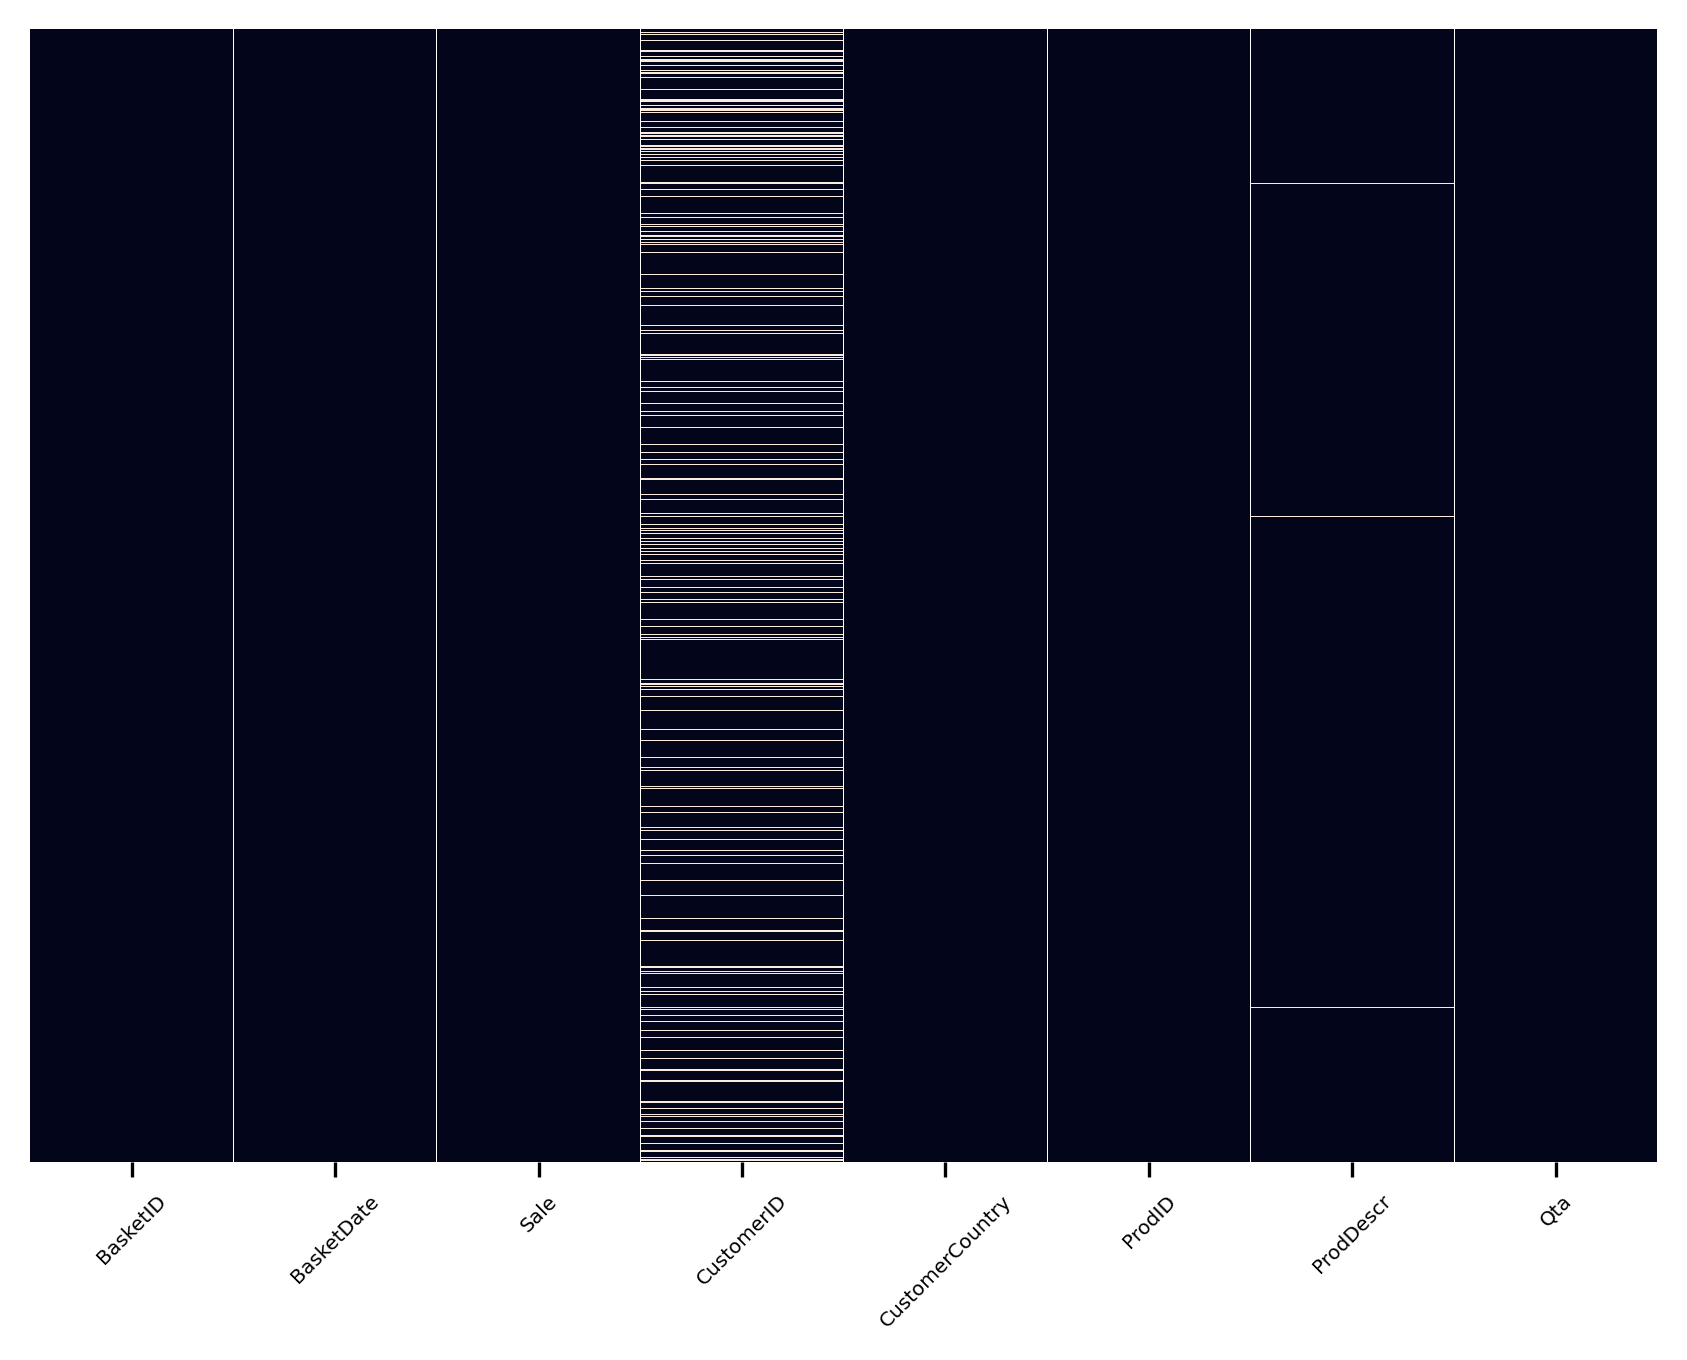
\includegraphics[height=9cm, width=15cm]{img/missing_values.png}
\caption{Missing values}
\end{figure}

We checked attributes like \textbf{BasketDate}, \textbf{Sale} and \textbf{Qta} to see if there were some syntactic errors, but we did not find any of them.

Afterwards, we checked the \emph{semantic accuracy} of the entries in the dataset, to see if some value was not coherent with the logic of its attribute.\\
In particular, we found:
\begin{itemize}
\item 2 records with a negative value for \textbf{Sale};

\item Some rows with "\emph{strange}" \textbf{ProdDescr}, not referring to a particular product
	\begin{itemize}
		\item Some of them describe the product's conditions, \emph{e.g.} '\emph{Damaged}', '\emph{wet rusty}', '\emph{Unsaleable destroyed}'. We noticed that these records have all \emph{NULL} \textbf{CustomerID}, so we consider these objects not as actual purchases, but instead as internal operations of the supermarket staff;
		\item Other ones are referring to some online buying, \emph{e.g.} '\emph{amazon}', '\emph{ebay}', '\emph{dotcom sales}', but we couldn't be able to understand the real meaning of these objects, since they are very few in the dataset;
		\item Others, like '\emph{Manual}' and '\emph{Next Day Carriage}', are related to some particular situations, that are not interesting in relation to our analysis;
	\end{itemize}

\item Some rows have negative values for \textbf{Qta}; here, we discover an interesting pattern: in fact, all the rows with a \textbf{BasketID} starting with \textbf{C}, have a negative \textbf{Qta}. We interpret these records as refunds.
\end{itemize}

\begin{wrapfigure}{r}{.5\textwidth}
\centering
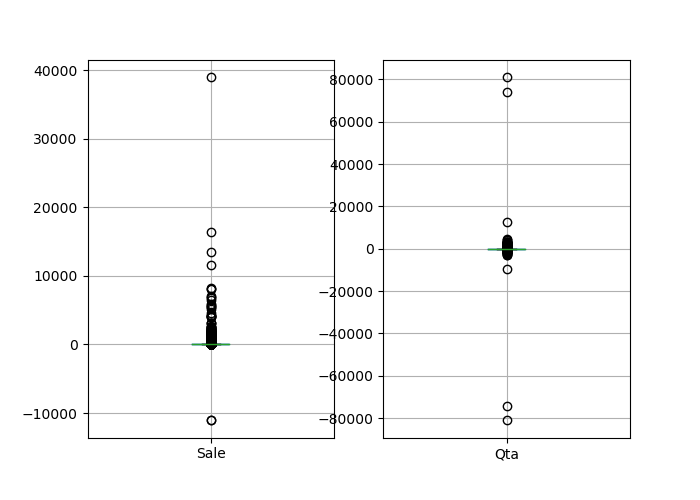
\includegraphics[width=0.49\textwidth]{img/boxplot_before.png}
\caption{Box Plot for outliers detection}
\end{wrapfigure}

For what regards the outliers, we used a box plot to visualize the two continuous attributes that we have, that are \textbf{Sale} and \textbf{Qta}.\\
From these plots, we found that, for both attributes, the box is very flat, meaning that the vast majority of the values fall in a small range. Nevertheless, there are several outliers, someone with a value really far away from the median; these values could represent an issue for the analysis we will perform. Plus, here we can notice the negative values we already found during the semantic analysis.

\subsection{Variables Transformations}
We chosen to categorize the attribute \textbf{BasketDate}, by first splitting the date information and the time information, and then

\begin{itemize}
\item for the time, we decided to divide the day hours into 5 categories:
	\begin{itemize}
	\item \emph{Early morning}, from 6 to 9;
	\item \emph{Morning}, from 9 to 12;
	\item \emph{Lunch time}, from 12 to 15;
	\item \emph{Evening}, from 15 to 18;
	\item \emph{Late evening}, from 18 to 21.
	\end{itemize}
\item for the date, we chosen to keep the week of the transaction.
\end{itemize}

The rationale behind these choices is that we are more interested in the period in which a transaction occurs, rather that its precise date and time, to be able to cluster customers with a similar shopping behavior; furthermore, since the dataset is not from a grocery store, the customers with several shopping sessions per day or per week are really rare, and so we decided to use a broader partitioning.\\
After these categorization, we ended introducing \textbf{DayTime} and \textbf{Week}.

We also decided to create the attribute \textbf{TotalPrice}, which is simply the product of \textbf{Sale} and \textbf{Qta}, and represents the total amount spent by a customer for each record. We made this choice mainly to have a clearer look to the dataset, emphasizing an important information that was not explicit in the original table, and also to simplify the extraction of some features and statistics.

\subsection{Variables Distribution}
In this section, we will study the distribution of various attributes, by plotting some interesting properties about them.

\begin{figure}[!h]
\begin{subfigure}{.5\textwidth}
\centering
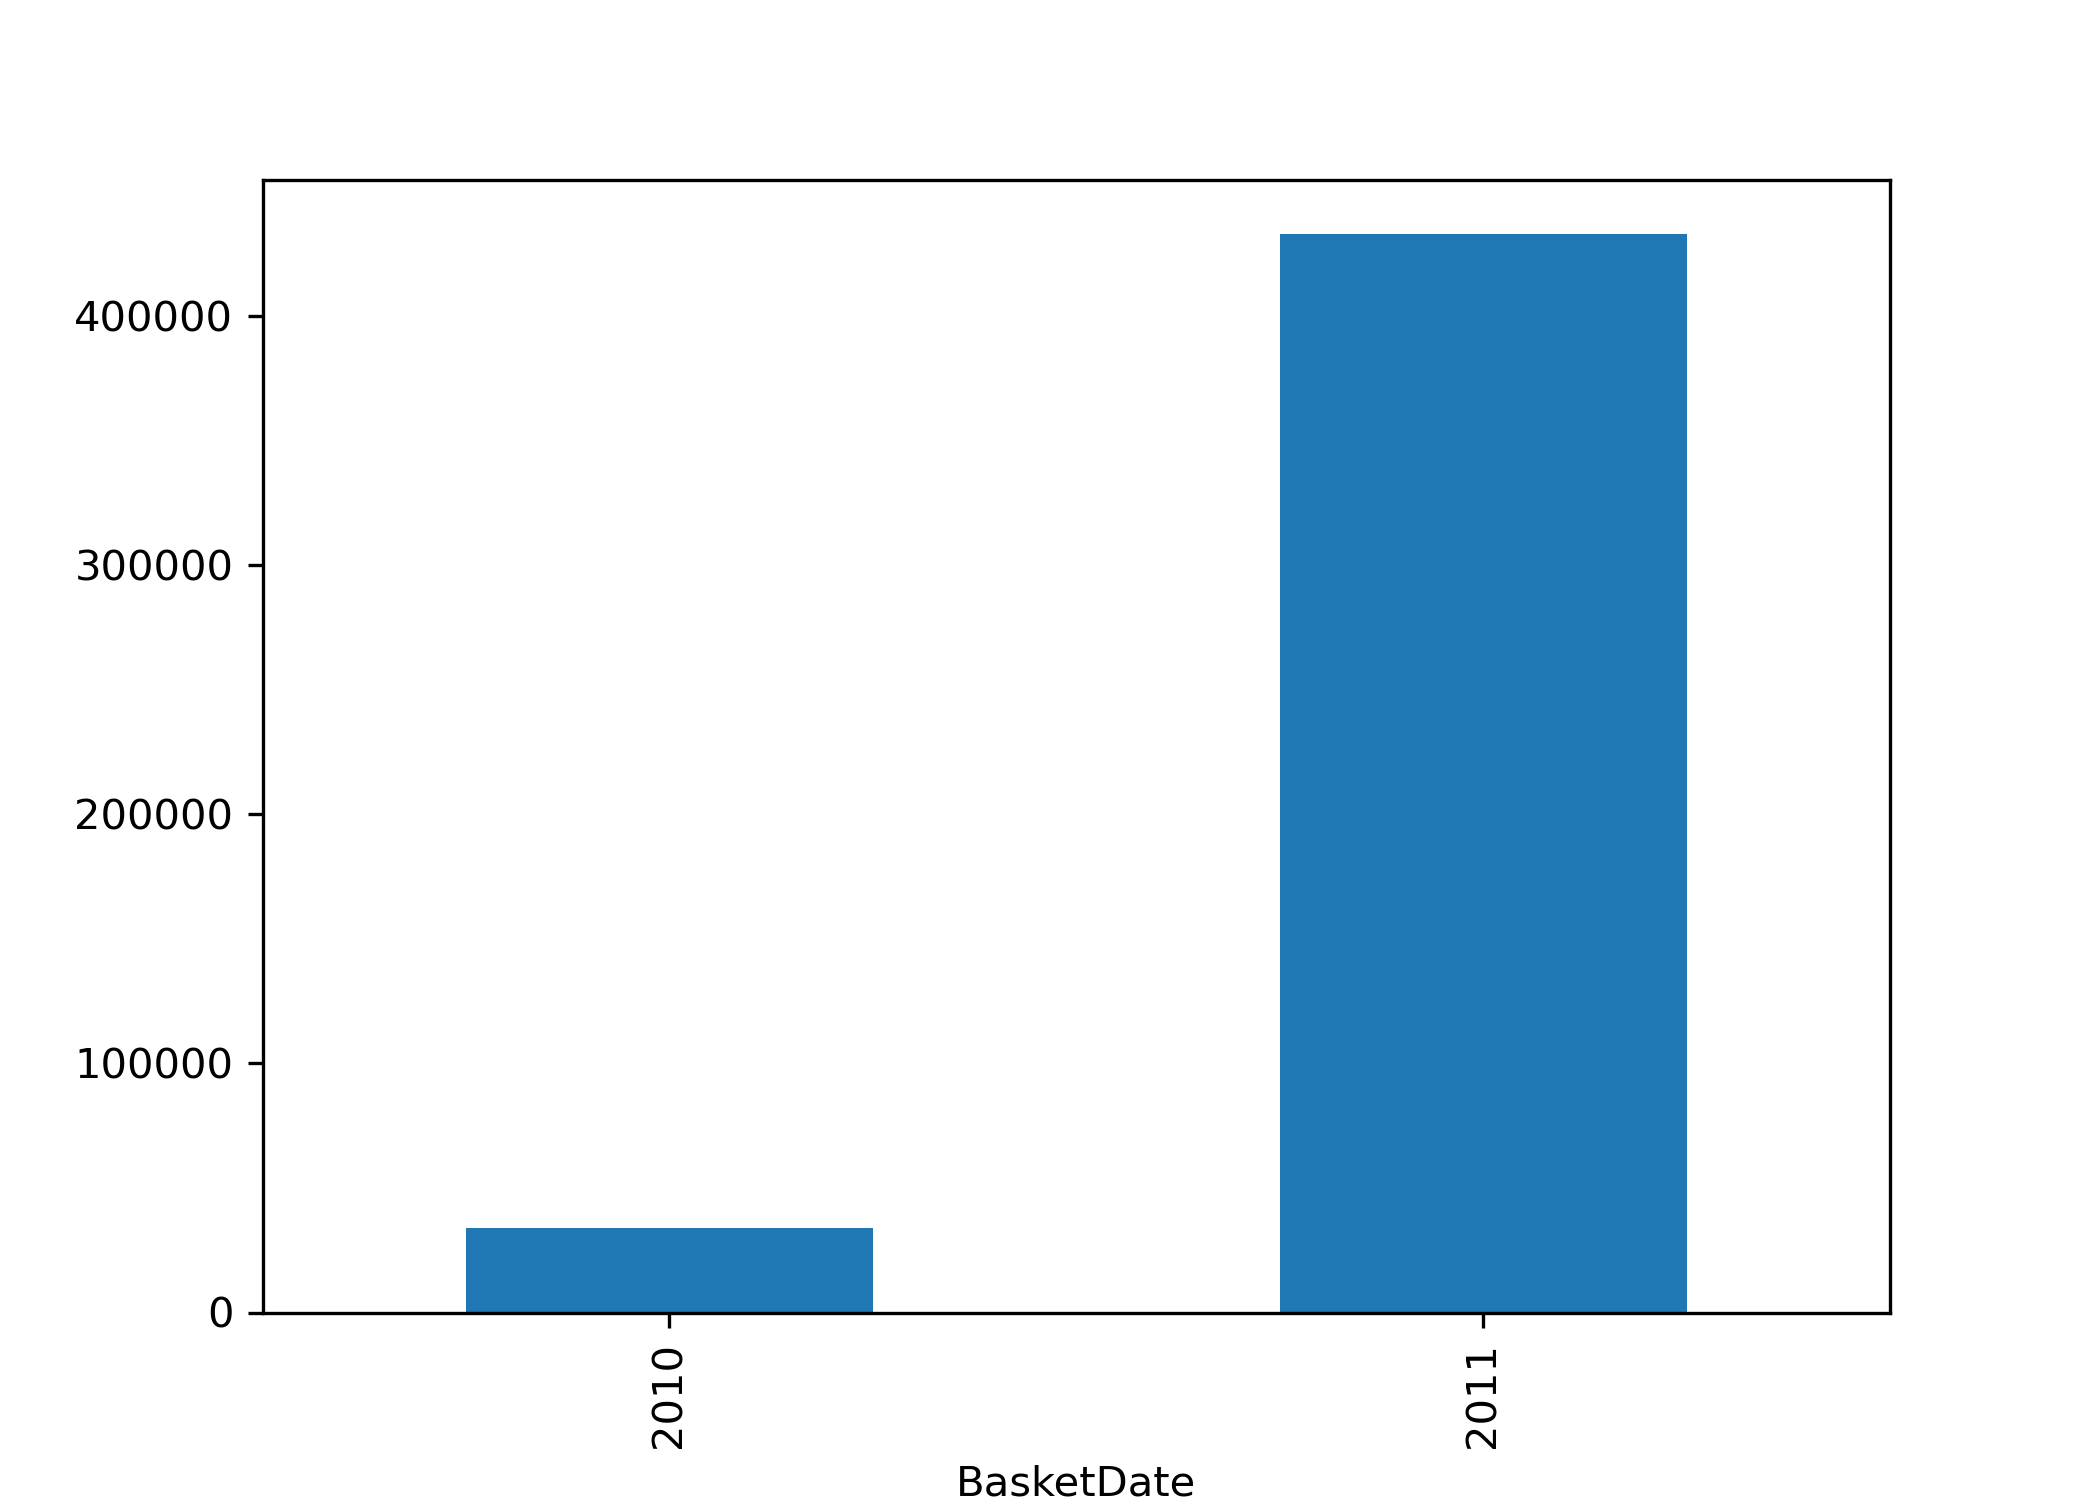
\includegraphics[width=.9\textwidth]{img/year_count.png}
\caption{Year}
\label{fig:year_count}
\end{subfigure}
\begin{subfigure}{.5\textwidth}
\centering
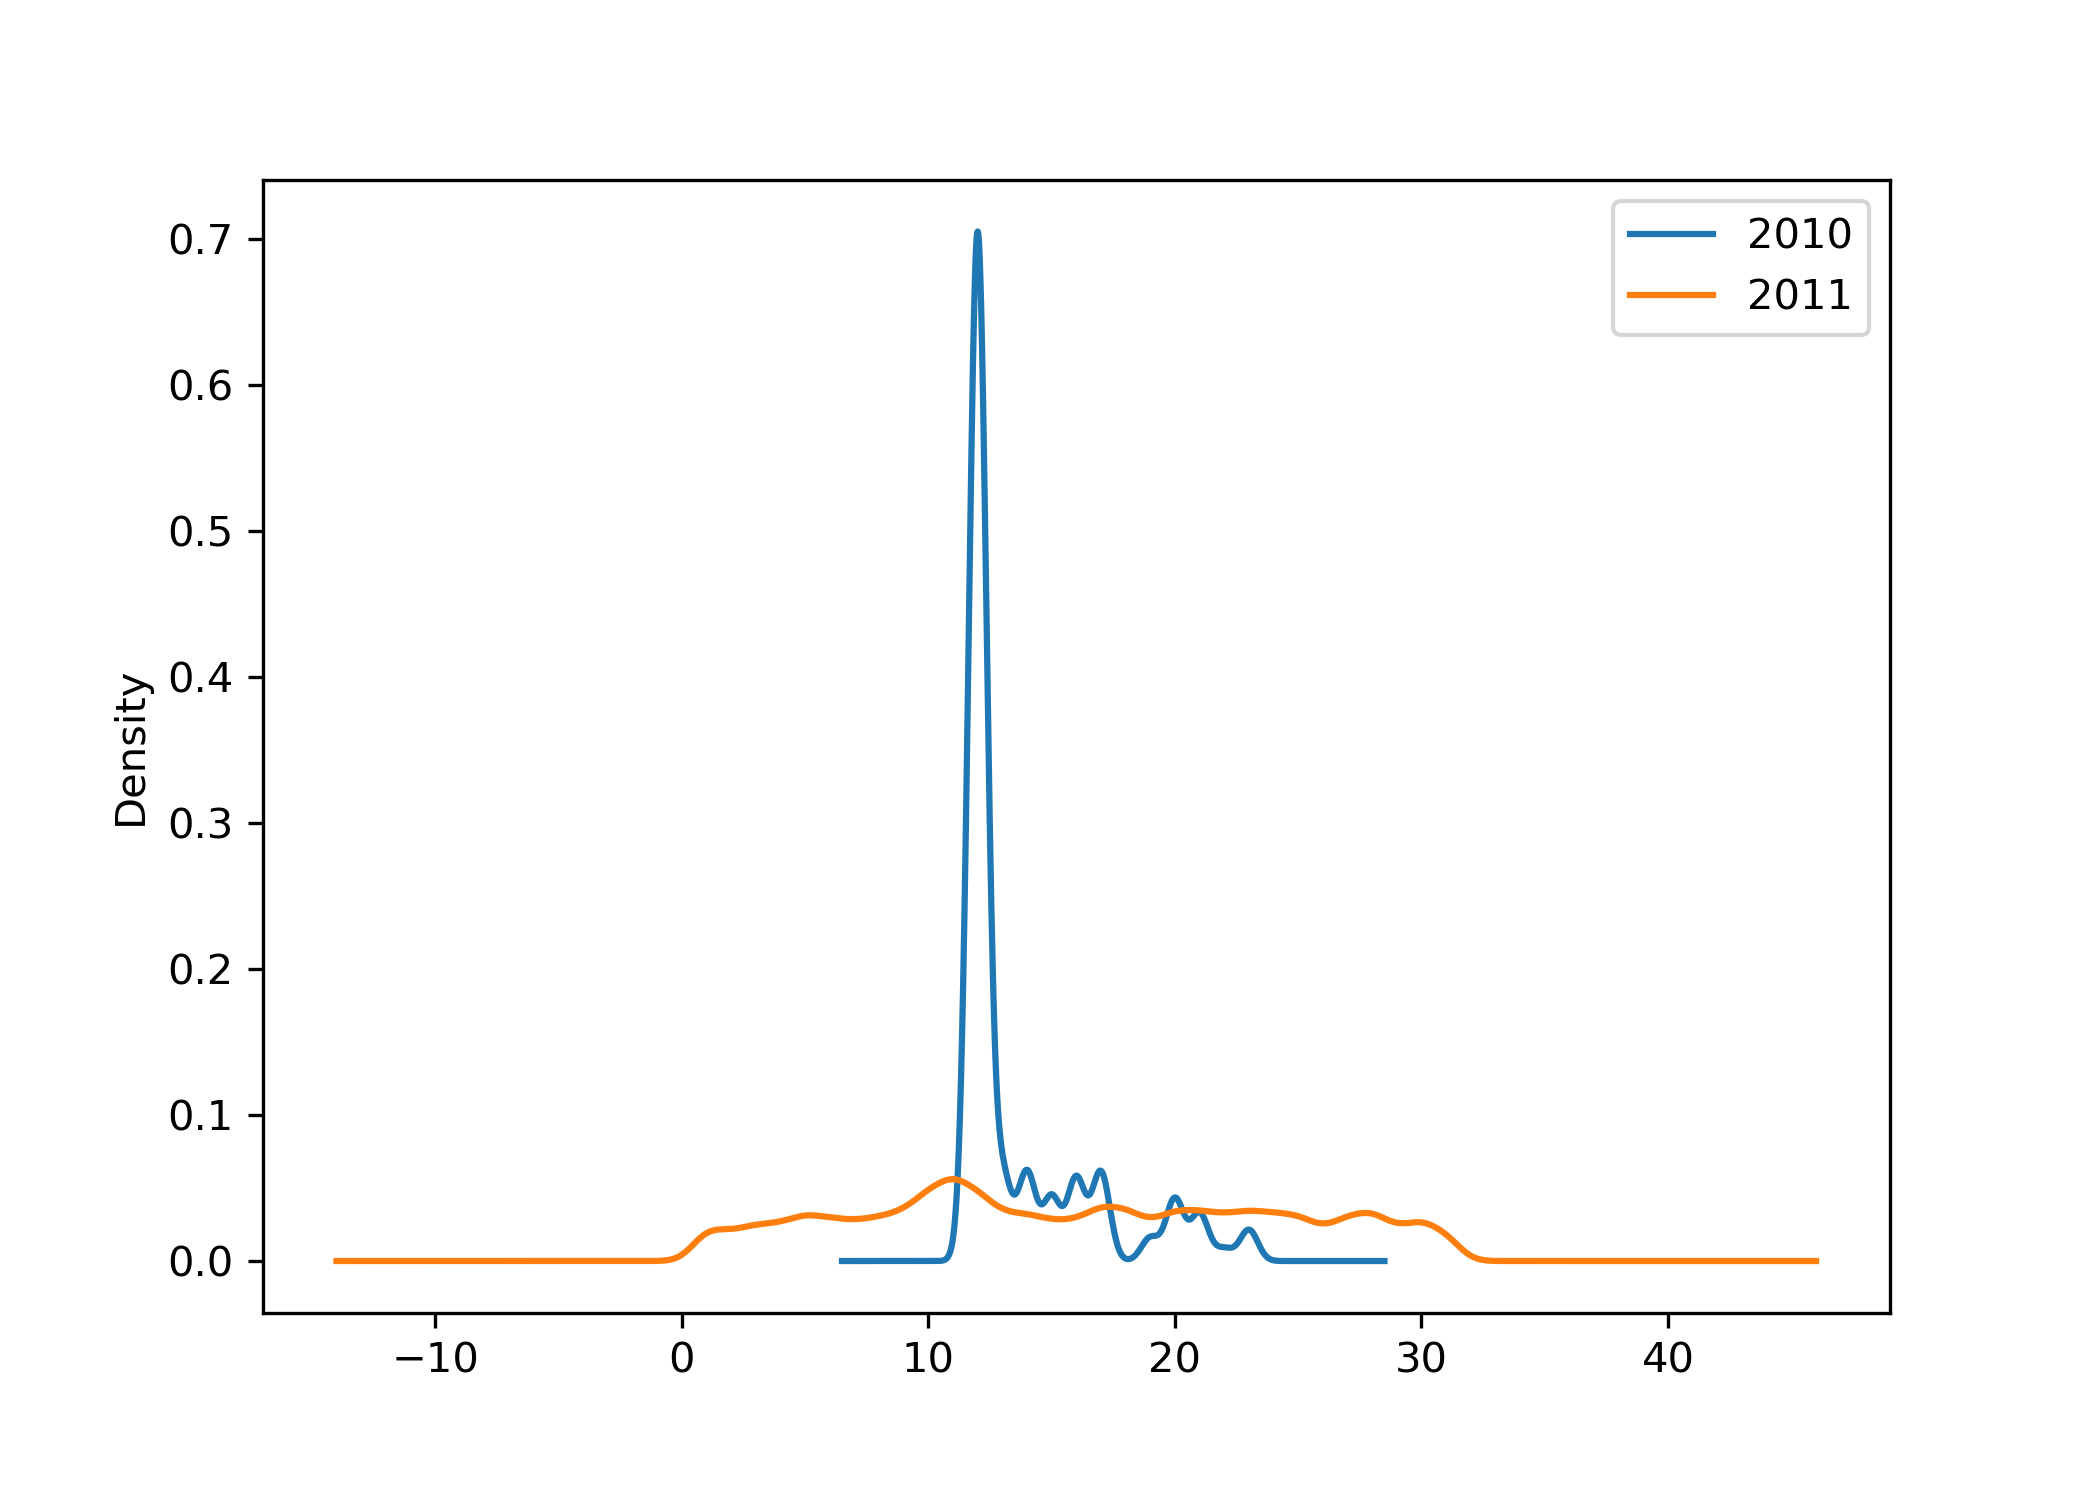
\includegraphics[width=.9\textwidth]{img/kde_year.png}
\caption{PDF by Year}
\label{fig:kde_year}
\end{subfigure}
\begin{subfigure}{.5\textwidth}
\centering
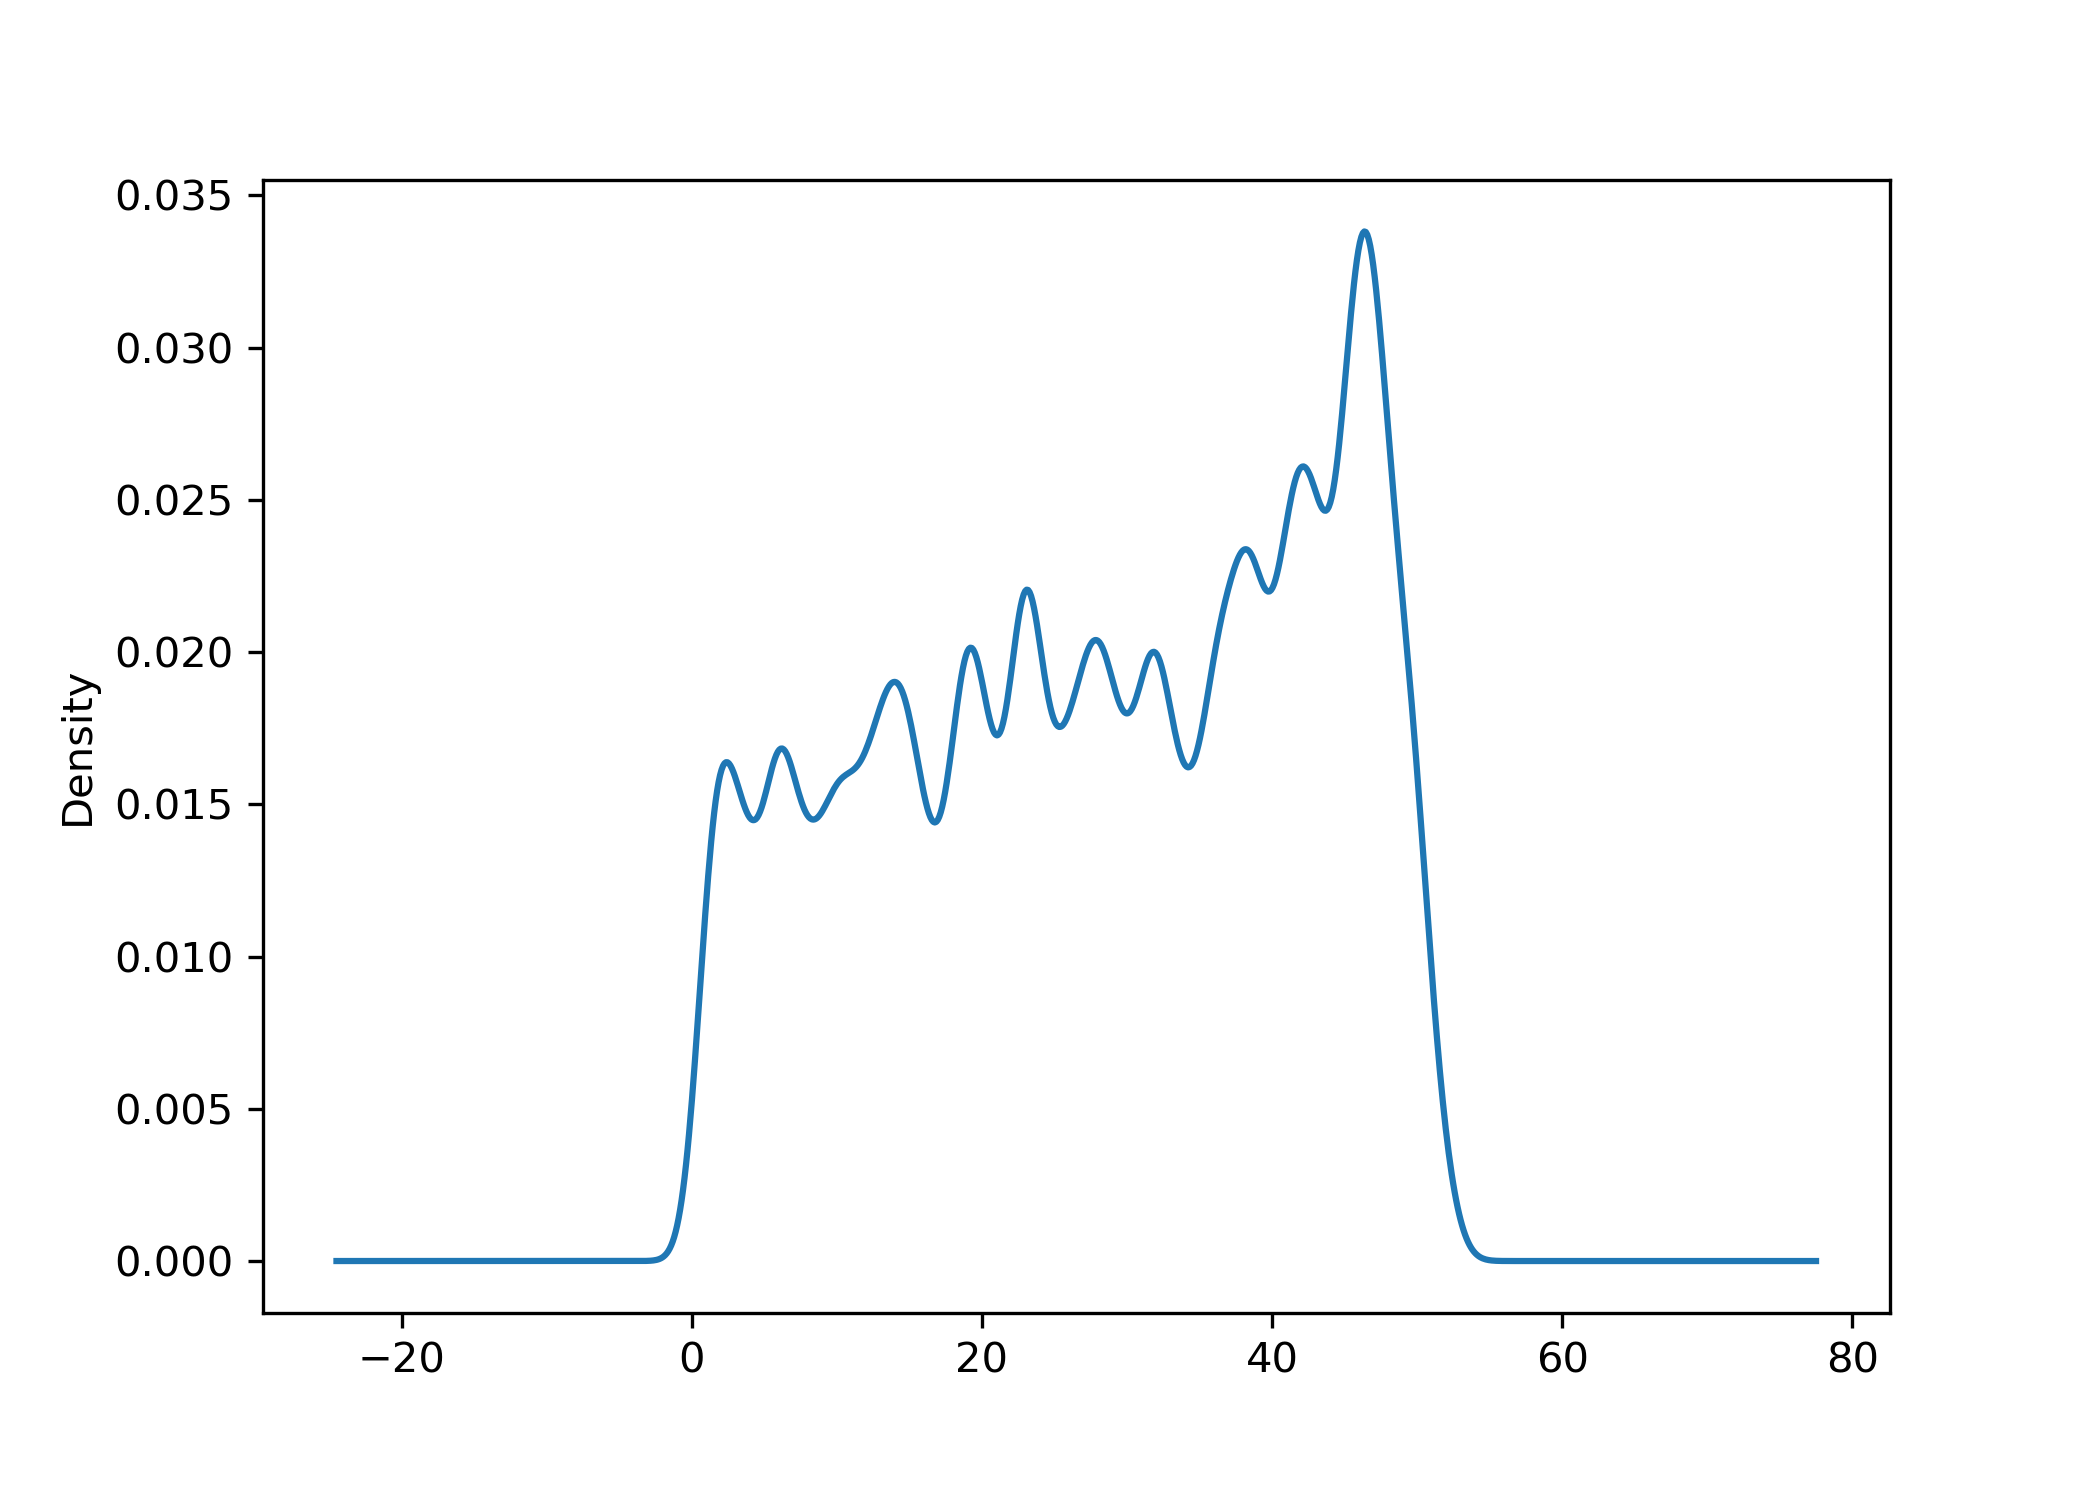
\includegraphics[width=.9\textwidth]{img/week_kde.png}
\caption{PDF by Week}
\label{fig:week_kde}
\end{subfigure}
\begin{subfigure}{.5\textwidth}
\centering
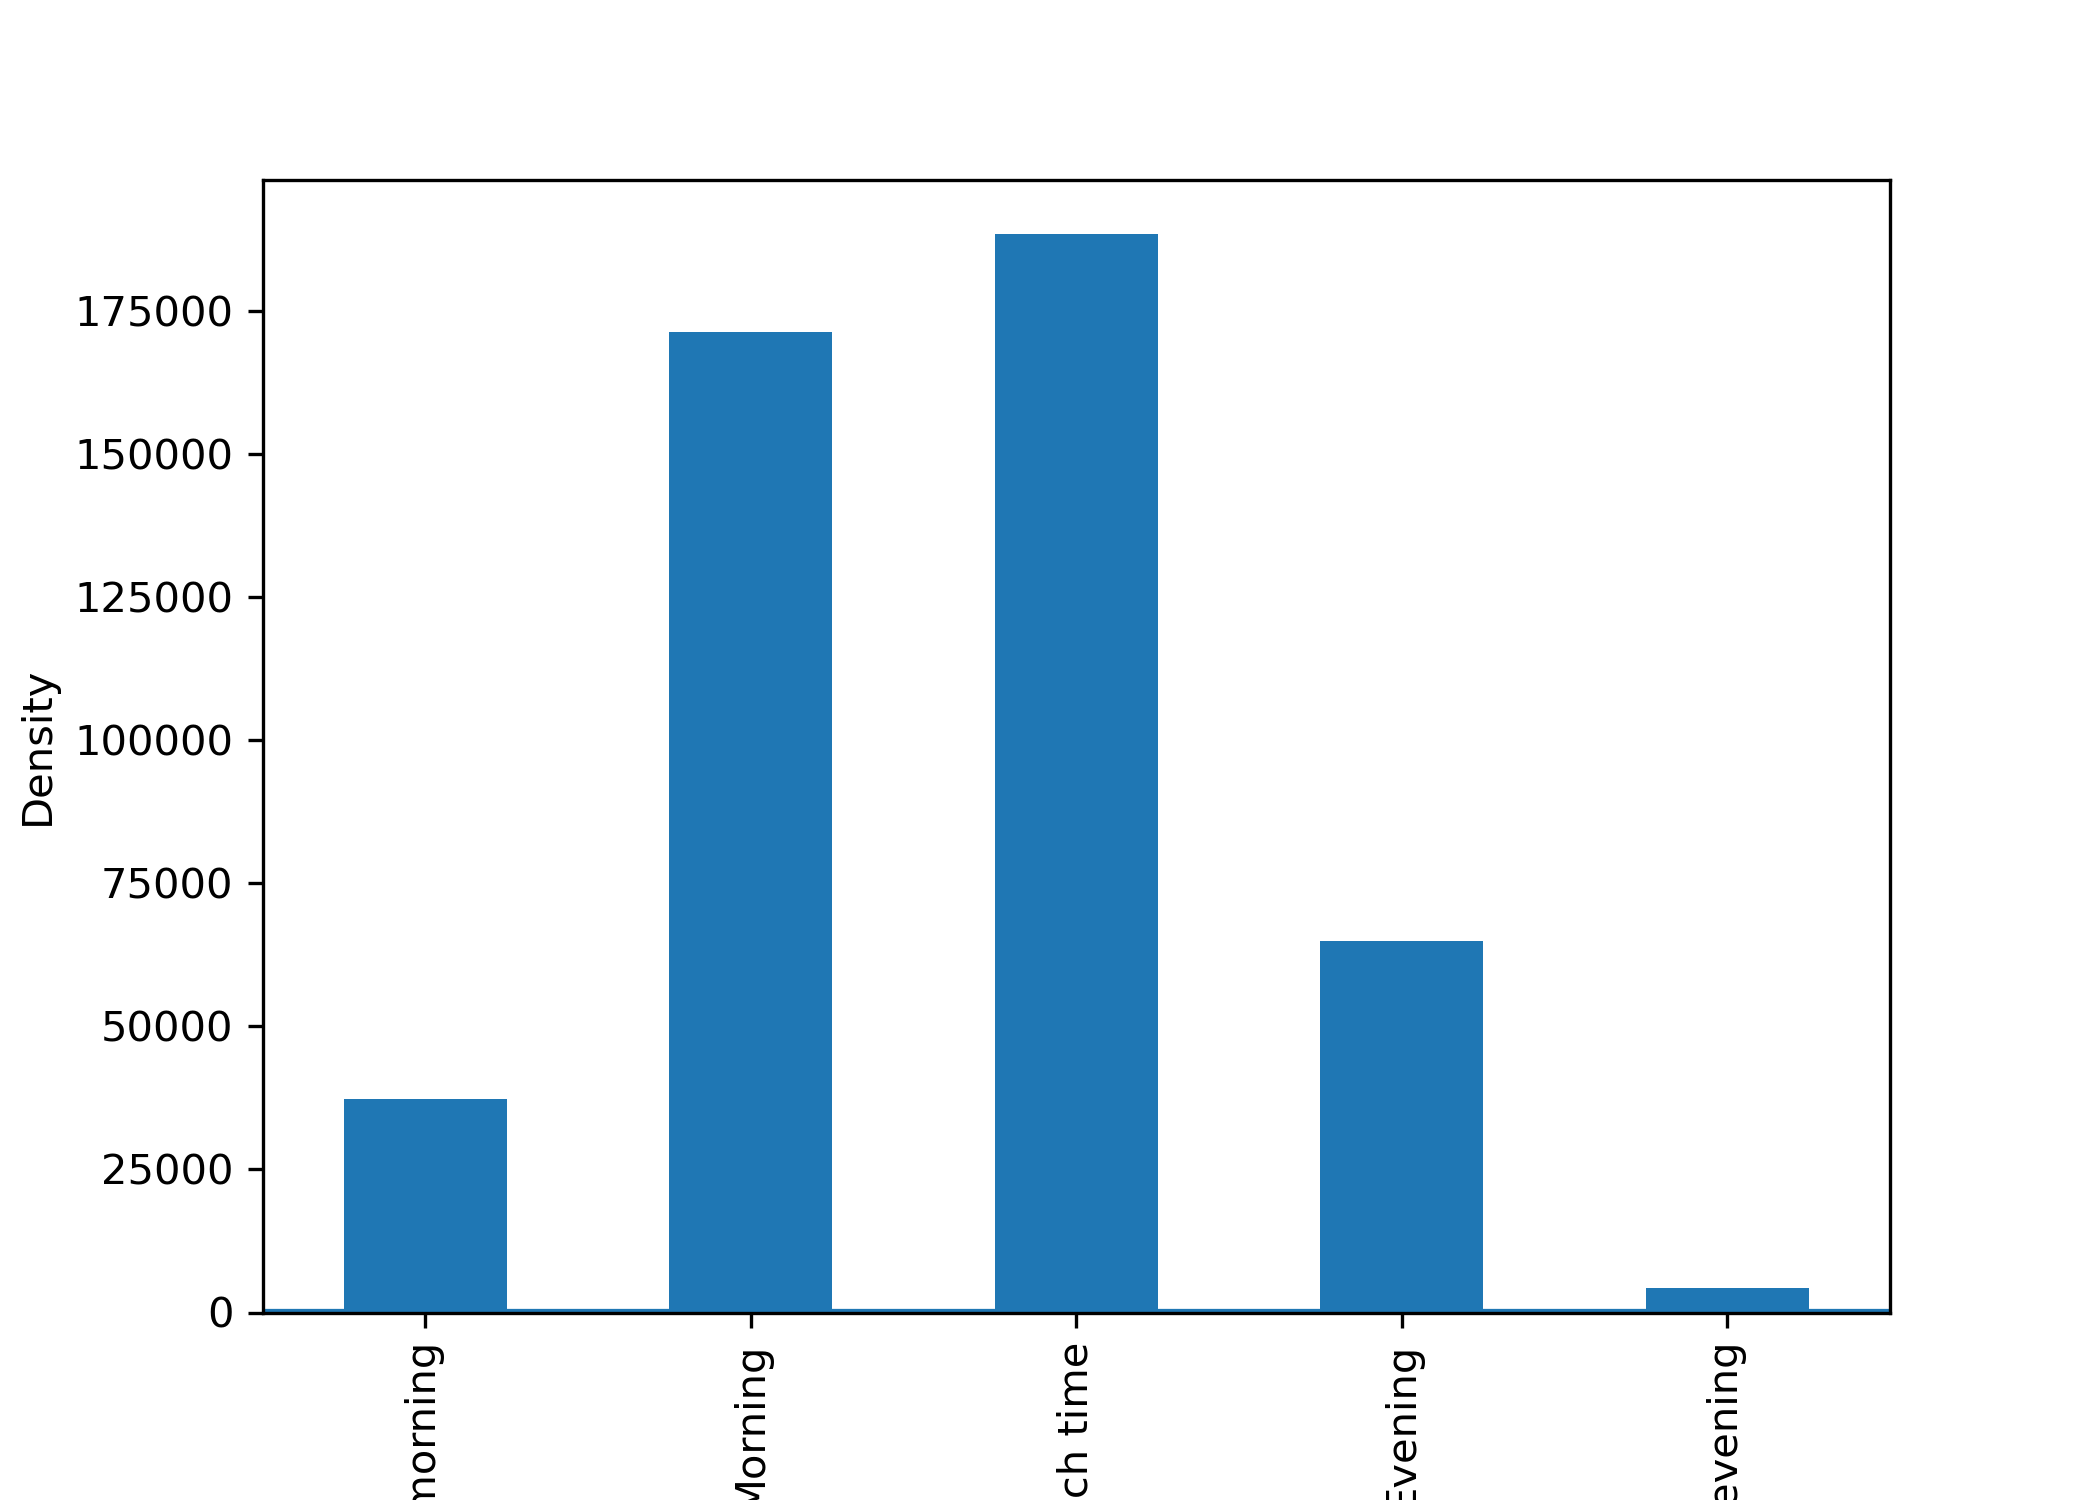
\includegraphics[width=.9\textwidth]{img/daytime_bar.png}
\caption{Day Time}
\label{fig:daytime_bar}
\end{subfigure}
\caption{BasketDate Distributions}
\end{figure}

First, we analyse the \textbf{BasketDate}.\\
From the Figure \ref{fig:year_count}, we can see that the attribute is highly unbalanced; in fact, we have that almost all the records are related to transaction of the 2011, while the objects from 2010 are very few.
Indeed, the rows of 2011 represent about the 93\% of the whole dataset.\\
Furthermore, from the Figure \ref{fig:kde_year}, that represents an estimation of the probability density function of \textbf{BasketDate} divided by year, we can appreciate the different distributions for the two years.\\
In fact, for the 2010, we have a very uneven plot, which indicates that the records are not uniformly distributed with respect to the days in a month. That is justified by the fact that, for the majority of the months in 2010, there were registered only transactions from a single day; this day, that is the 12th, is the value for which the plot shows the peak.\\
On the other hand, the distribution for the 2011 is much more homogeneous, meaning that the transactions were registered for most days in the months of that year.\\
Another interesting distributions are plotted in Figure \ref{fig:week_kde} and \ref{fig:daytime_bar}.\\
In the first one, we can see that the last weeks of the year are the one with more purchases; that is consistent with our knowledge, since those are the weeks closest to Christmas time, that typically represents a great period of shopping.\\	
In the second one, the focus is instead on the hours in a day; we found that, unsurprisingly, the most popular hourly range goes from 9 to 18.

\begin{figure}[!h]
\begin{subfigure}{.5\textwidth}
\centering
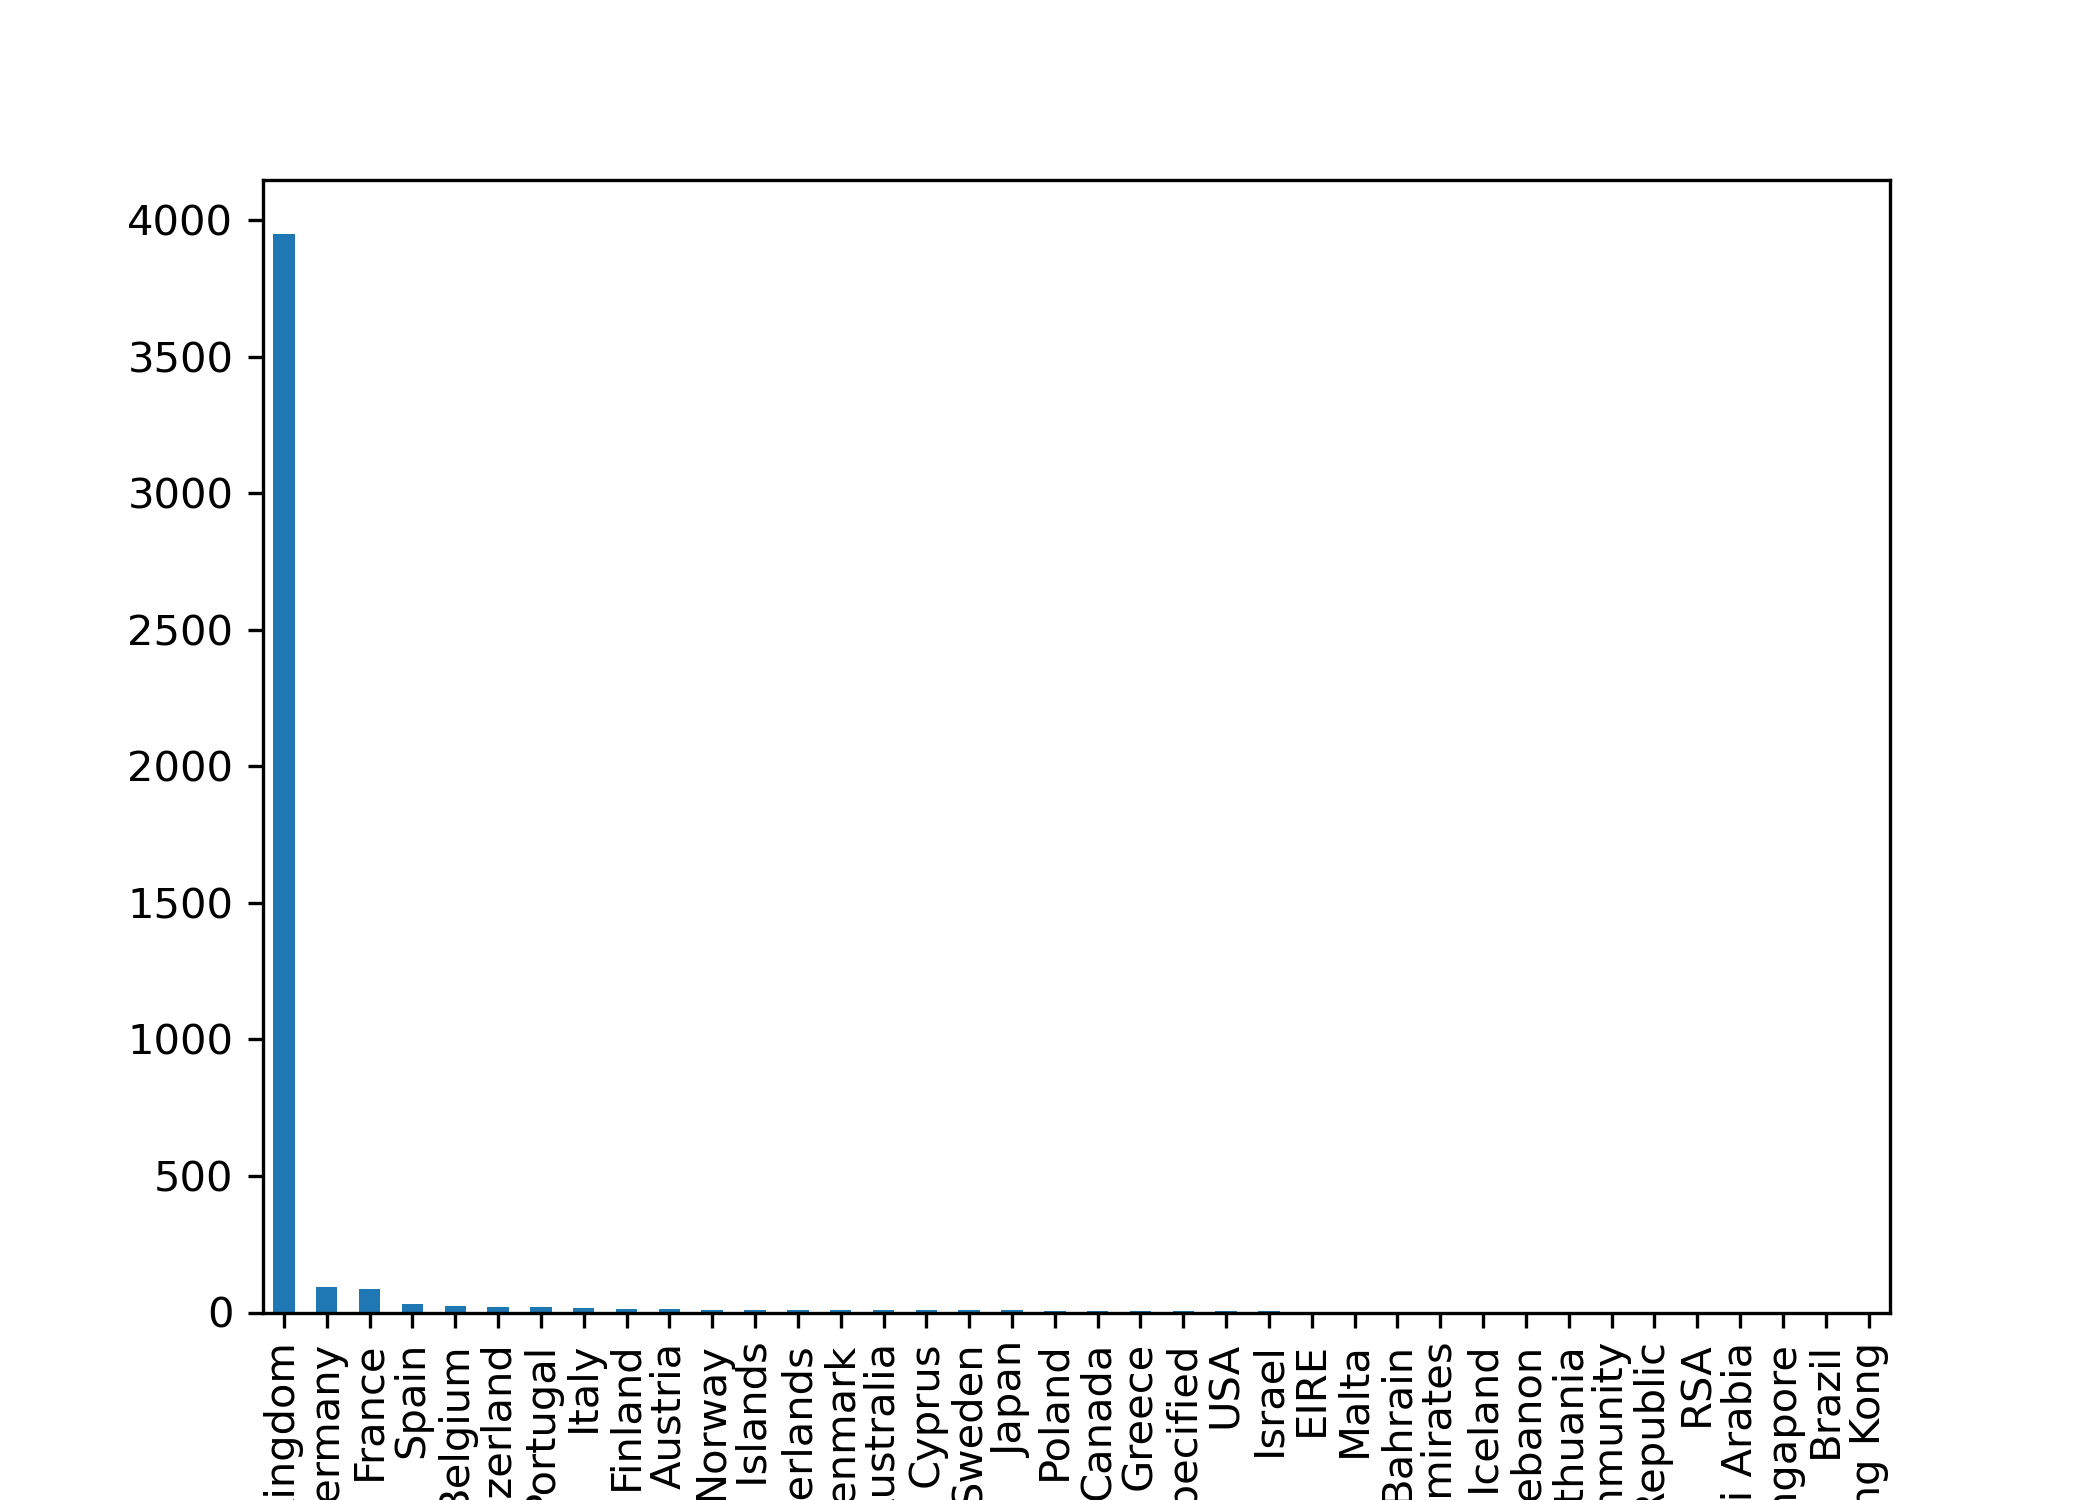
\includegraphics[width=\textwidth]{img/country_bar.png}
\caption{}
\label{fig:country_bar}
\end{subfigure}
\begin{subfigure}{.5\textwidth}
\centering
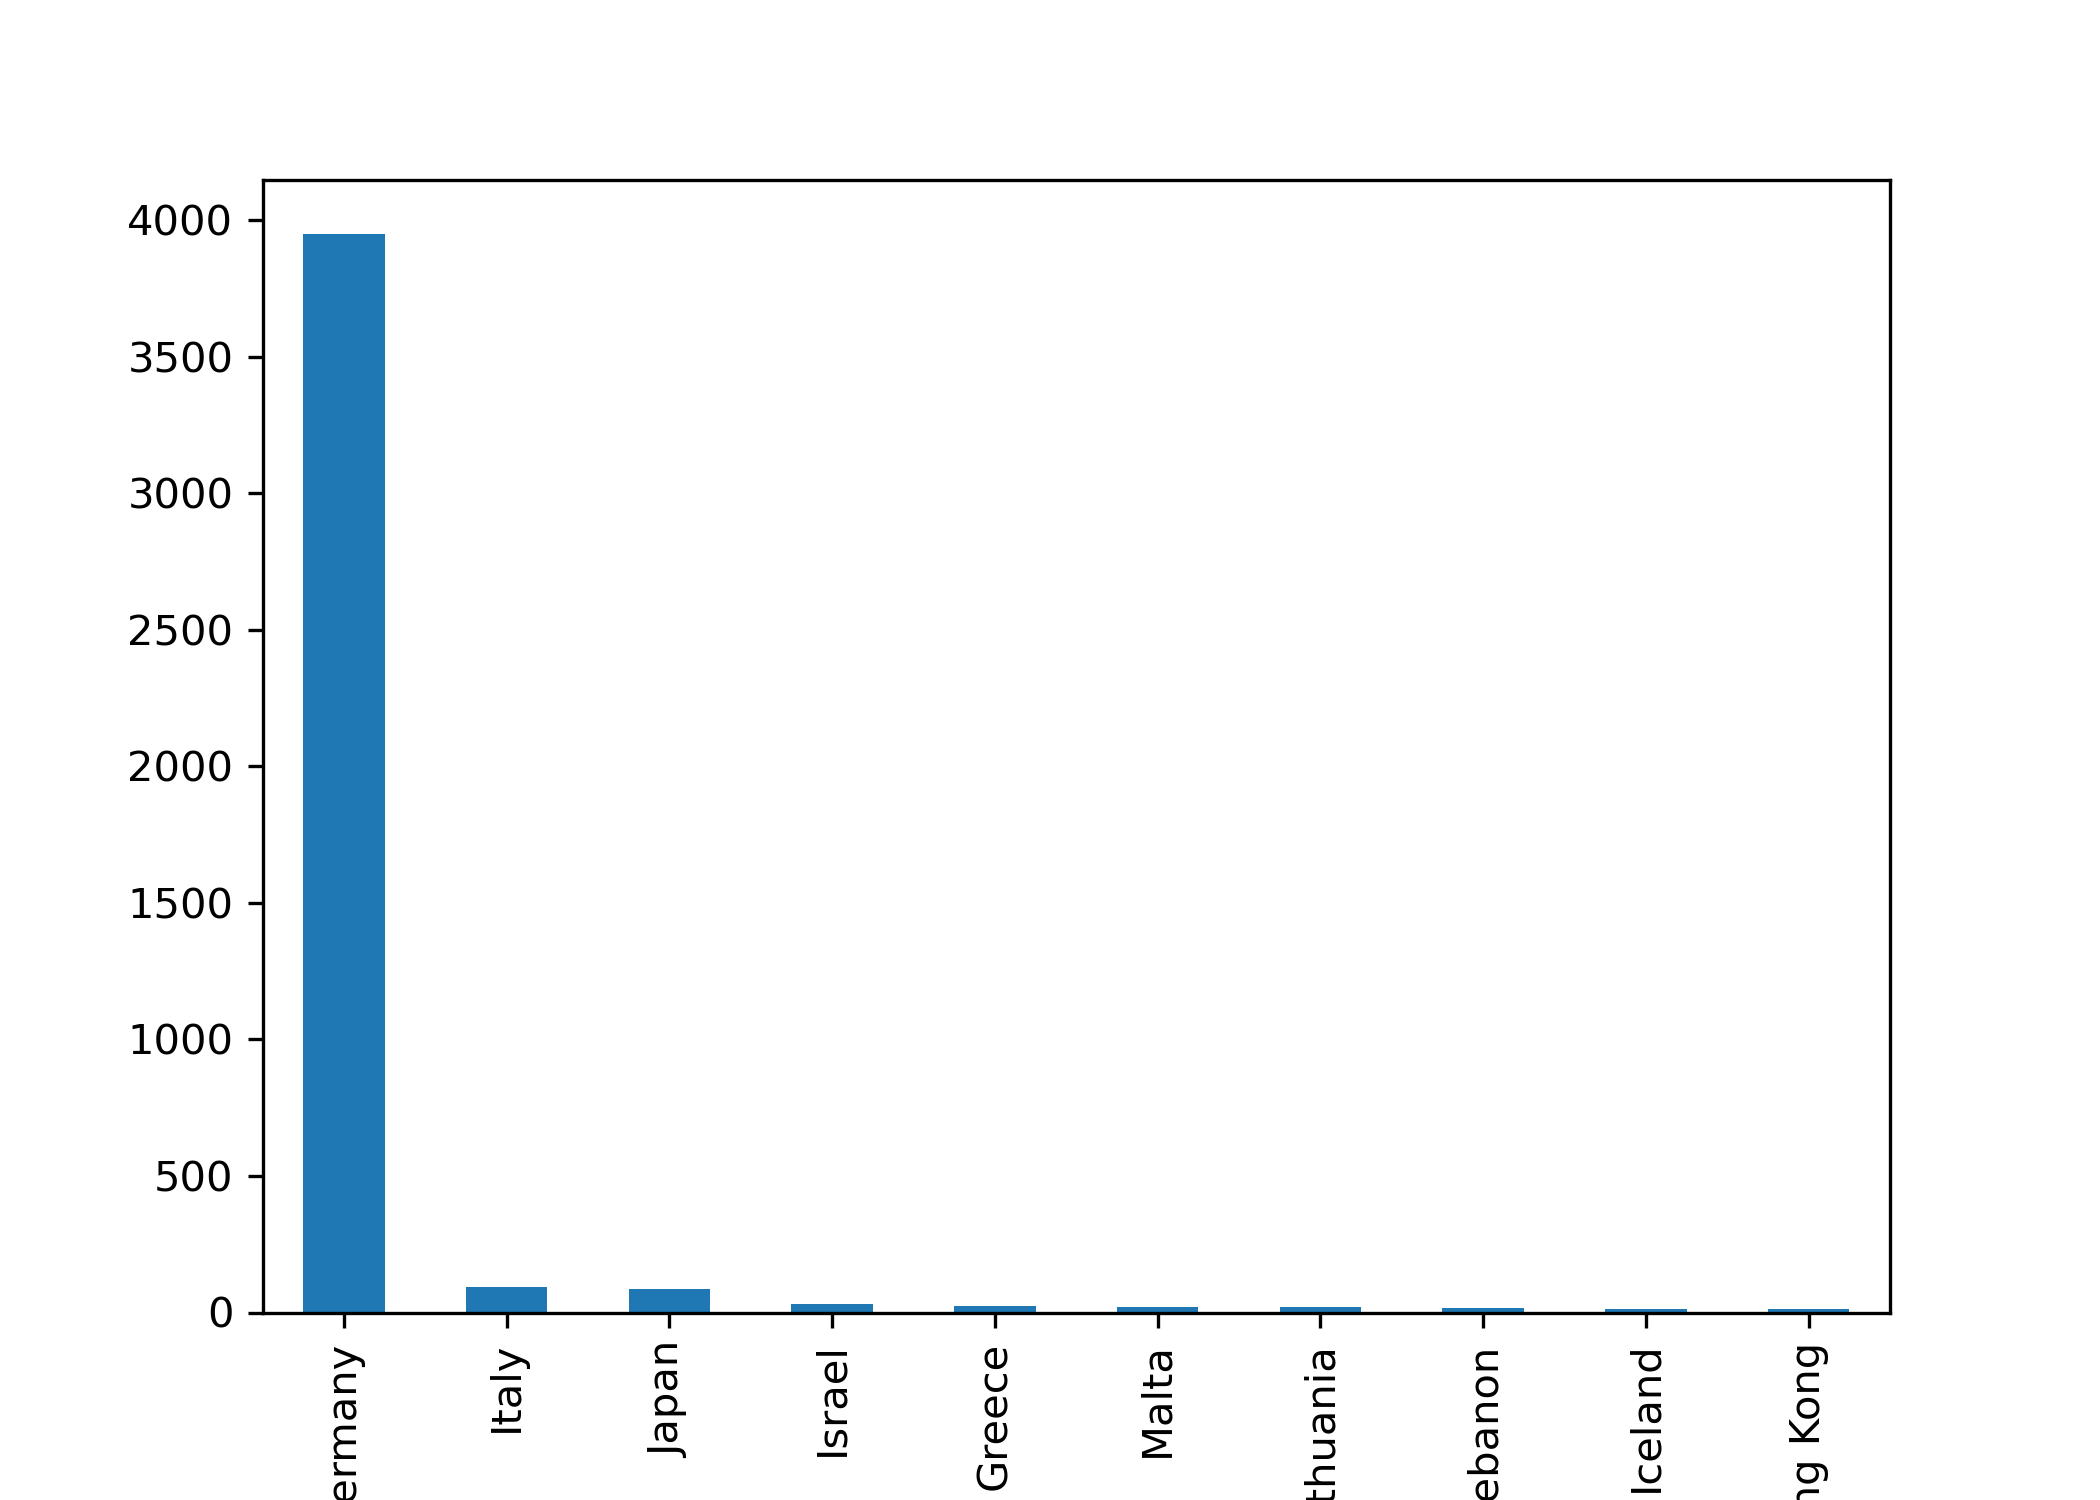
\includegraphics[width=\textwidth]{img/part_country_bar.png}
\caption{}
\label{fig:part_country_bar}
\end{subfigure}
\caption{CustomerCountry Distributions}
\end{figure}

Some others statistics can be visualized for the attribute \textbf{CustomerCountry}.\\
In Figure \ref{fig:country_bar}, we can see the distribution of the CustomerID with respect to the country; from the plot, it is clear that the most frequent country is the United Kingdom, that is present in about the 90\% of the rows.\\
To see also some properties of the other countries, in Figure \ref{fig:part_country_bar}, we plotted the most frequent countries, excluding the UK. Here, we can see that the second most frequent country is Germany, while the other ones are almost irrelevant, since they are in very few objects.

\begin{wrapfigure}{r}{.5\textwidth}
\centering
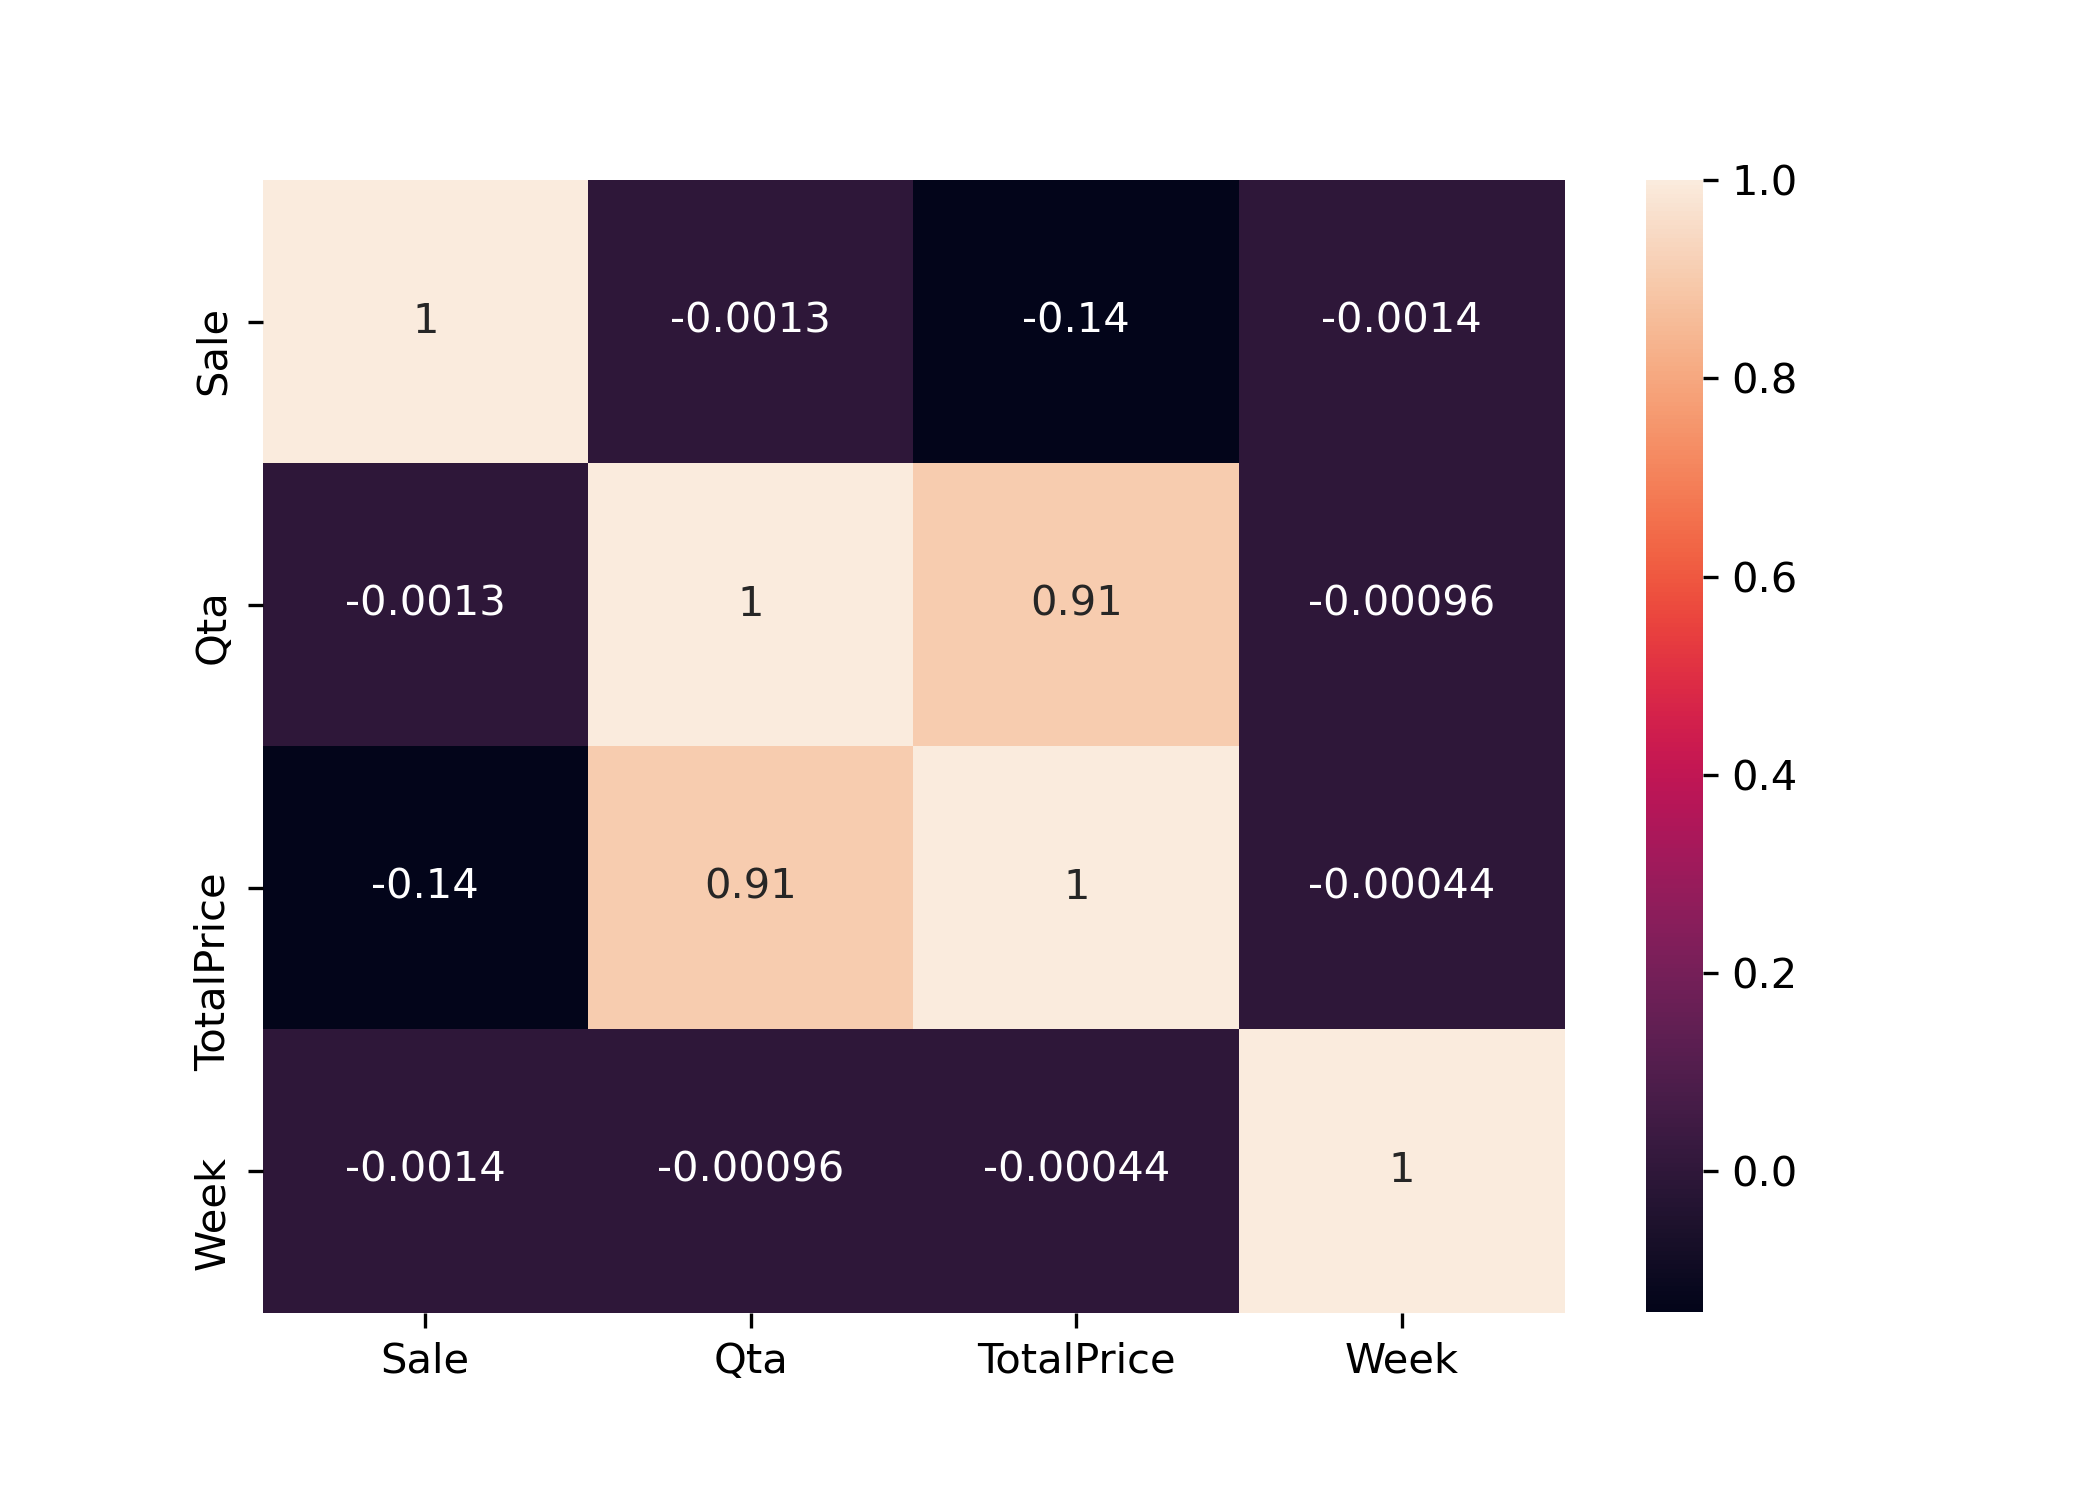
\includegraphics[width=0.49\textwidth]{img/corr.png}
\caption{Correlation Matrix}
\label{fig:corr}
\end{wrapfigure}

Finally, we see some informations about the correlation of the attributes, to see if some of them are redundant.\\
From the Figure \ref{fig:corr}, we can see that almost all the attributes are uncorrelated, except for \textbf{TotalPrice}, that shows ah high correlation with \textbf{Qta}; that follows what we expected, since \textbf{TotalPrice} is, by construction, dependent on \textbf{Qta}. So, we conclude that all the original columns are independent, and so we don't need to perform any further manipulation.
